%%%%%%%%%%%%%%%%%%%%%%%%%%%%%%%%%%%%%%%%%%%
%%% DOCUMENT PREAMBLE %%%
\documentclass[12pt]{report}
\usepackage[english]{babel}
\usepackage{hyperref}
%\usepackage{natbib}
\usepackage{url}
\usepackage[utf8x]{inputenc}
\usepackage{amsmath}
\usepackage{relsize}
\usepackage{graphicx}
\usepackage{physics}
\usepackage{adjustbox}
\graphicspath{{images/}}
\usepackage{parskip}
\usepackage{fancyhdr}
\usepackage{vmargin}
\setmarginsrb{3 cm}{2.5 cm}{3 cm}{2.5 cm}{1 cm}{1.5 cm}{1 cm}{1.5 cm}

\title{1}								
% Title
\author{ EP4031}						
% Author
\date{today's date}
% Date

\makeatletter
\let\thetitle\@title
\let\theauthor\@author
\let\thedate\@date
\makeatother

\pagestyle{fancy}
\fancyhf{}
\rhead{\theauthor}
\lhead{\thetitle}
\cfoot{\thepage}
%%%%%%%%%%%%%%%%%%%%%%%%%%%%%%%%%%%%%%%%%%%%
\begin{document}

%%%%%%%%%%%%%%%%%%%%%%%%%%%%%%%%%%%%%%%%%%%%%%%%%%%%%%%%%%%%%%%%%%%%%%%%%%%%%%%%%%%%%%%%%

\begin{titlepage}
	\centering
    \vspace*{0.5 cm}
   % \includegraphics[scale = 0.075]{bsulogo.png}\\[1.0 cm]	% University Logo
\begin{center}    \textsc{\Large   Data Science Analysis}\\[2.0 cm]	\end{center}
	\textsc{\Large EP4130 | IIT Hyderabad  }\\[0.5 cm]				% Course Code
	\rule{\linewidth}{0.2 mm} \\[0.4 cm]
	{ \huge \bfseries Stock Market Analysis}\\
	\rule{\linewidth}{0.2 mm} \\[1.5 cm]
	
	\begin{minipage}{0.4\textwidth}
		\begin{flushleft} \large
		%	\emph{Submitted To:}\\
		%	Name\\
          % Affiliation\\
           %contact info\\
			\end{flushleft}
			\end{minipage}~
			\begin{minipage}{0.4\textwidth}
            
			\begin{flushright} \large
			\emph{} \\
                Gautham Gururajan \\ 
                Raghav Girgaonkar
		\end{flushright}
           
	\end{minipage}\\[2 cm]
	
% 	\includegraphics[scale = 0.5]{PICMathLogo.png}
    
    
    
    
	
\end{titlepage}

%%%%%%%%%%%%%%%%%%%%%%%%%%%%%%%%%%%%%%%%%%%%%%%%%%%%%%%%%%%%%%%%%%%%%%%%%%%%%%%%%%%%%%%%%

\tableofcontents
\pagebreak

%%%%%%%%%%%%%%%%%%%%%%%%%%%%%%%%%%%%%%%%%%%%%%%%%%%%%%%%%%%%%%%%%%%%%%%%%%%%%%%%%%%%%%%%%
\renewcommand{\thesection}{\arabic{section}}
\section{Abstract}
 
 Often, we find ourselves doubting the existence of real world applications of Data Analysis Theory, as it is not trivial to understand what how and where the standard tools are used 
 
 This paper aims to capture that very essence by making use of some known data analysis tools to help make predictions and inferences for and of the stock market.
 
 We have chosen the stock market as there exists an abundance of data to check and validate certain hypotheses, and to analyze it, we have chosen the Neural Network prediction system.

Here, we have chosen to analyze the S\&P 500, which is an American stock market index based on the market capitalizations of 500 large companies having common stock listed on the NYSE, NASDAQ, or the Cboe BZX Exchange.


\newpage
\section{Introduction}
The S\&P 500 is an American stock market index consisting of the market capitalizations of 500 large companies listed on the NYSE, NASDAQ, or the Cboe BZX Exchange.

We acquired a dataset which consisted of the S\&P 500 index along with the stock prices of the 500 companies. The data samples present in the data were minute-by-minute stock prices of all the 500 companies which include Apple, Boeing Company and the Goldman Sachs Group. In this project we have built a deep learning model in Tensor-Flow to predict the S\&P 500 index using the data of the given 500 hundred companies.  
The data was properly cleaned and prepared by filling NaN values with LOC (Last Observation Carried forward) to ensure there were no gaps in the dataset.

Dataset can be seen in Figure 1.
\\ \\ \\ \\ 
\begin{adjustbox}{center,caption={First 5 rows and 6 columns of the dataset},label={somelabel},nofloat=figure,vspace=\bigskipamount}
% maybe other stuff
\includegraphics[scale = 0.6]{/home/raghav/Desktop/stockprediction/02_code/data2.eps}% example only, could also be \adjustimage
% maybe other stuff
\end{adjustbox}


% Dude upload the image directly here, check the images folder

%\begin{figure}
%\includegraphics[scale=0.6]{/home/raghav/Desktop/stockprediction/02_code/data2.eps}
%\caption{First 5 rows and 6 columns of the dataset}
%\end{figure}
\newpage
\section{The BP Neural Network}

The \textit{Back Propagation Neural Network}, is an extremely popular method used for prediction models. In this type of neural network, the inputs which are fed in, are propogated in the forward direction and then compared with the actual values which should be obtained. After this the \textit{weights} of each of its \textit{layers} are changed by a reverse process known as \textit{backpropogating}. Thus the neural network \textit{learns} after every batch of input is passed through it and corrects itself by adjusting its \textit{weights} accordingly.


\subsection{Basic Terminology}
\subsubsection{Neuron}
The word \textit{neuron} is inspired by the biological neuron present in our bodies as it performs the same function. Neurons pass on information in the form of electric signals in our body and similiarly in our neural network, a \textit{neuron} accepts inputs and their weights and gives the corresponding output according to the \textbf{\textit{Activation Function.}} 

\subsubsection{Bias}
A bias unit is an "\textit{extra}" neuron added to each pre-output layer that stores the value of 1. Bias units aren't connected to any previous layer and in this sense don't represent a true "\textit{activity}". A bias is introduced as an input to represent what the neural network will output when no inputs are given to it.

\subsubsection{Activation Function}
The activation function decides, whether a neuron should be activated or not by calculating weighted sum and further adding bias with it. The purpose of the activation function is to introduce non-linearity into the output of a neuron.
\begin{figure}
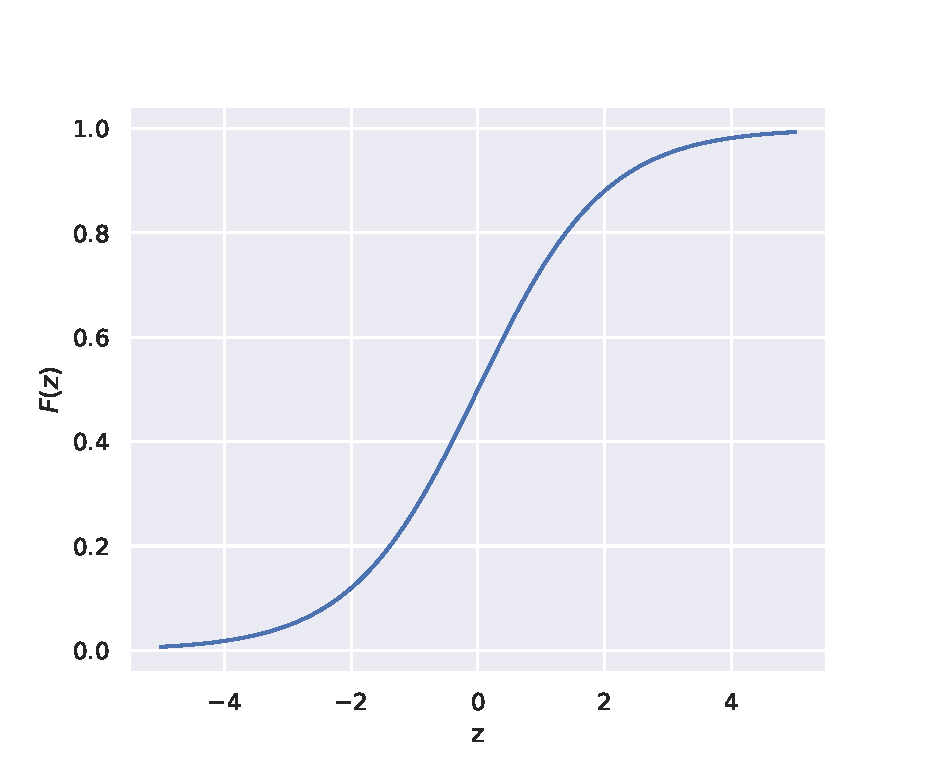
\includegraphics[scale=0.6]{/home/raghav/Desktop/stockprediction/02_code/afunc.eps}
\caption{Activation Function: Sigmoid Function}
\end{figure}

\subsection{Working}

A Neural Network is usually made up of multiple layers.
Of course, one input and one output layer, and included are one or many hidden layers for the purpose of filtering the data in a sense.

Let us assume a case of a total of $M$ layers where $m = 1$ represents the first layer(Input) and $m = M$ represents the last layer(Output).

We shall use $w^m_{jk}$ to denote the weight for the connection made between the $k$th neuron in the $(m-1)$th layer to the $j$th neuron in the $m$th layer.

Also, we use $b^m_j$ for the bias of the $j$th neuron in the $m$th layer, and for the activation of the $j$th neuron in the $m$th layer, we use $a_j^m$

Further, the activation $a_j^m$ is defined as 
\\ \\ 
$a_j^m$ = $\sigma\bigg(\sum_{k = 0} w^m_{jk}*a_{j-1}^k + b^m_j\bigg)$
\\ \\
where $\sigma$ is the activation function.
\\ \\
This then propogates in the forward direction of the neural network and the weights of each neuron in every layer is determined, this is called \textit{Forward Propogation}.
\\ \\
The Cost Function is calculated as follows \\ \\
$C$‎ ‎=‎ $\frac{1}{2n}\mathlarger{\mathlarger{‎‎\sum}}_{x}||y(x) - a_{L}(x)||^2$ = $\frac{1}{n}\mathlarger{\mathlarger{‎‎\sum}}_{x}C_x$
\\ \\
We then use the \textit{Hadamard Product} to calculate the intermediate error function $\delta$ \\ \\
$\delta^L$ = $\nabla_a C \odot \sigma^{'}(z^L)$ where $z^l$ = $w^{l}a^{l-1} + b^{l}$
\\ \\ 
With learning rates $\eta$ the weights are learned as follows \\ \\
$w^m_{jk}\rightarrow w^m_{jk} -\eta \pdv{C}{w^m_{jk}} $ and \\ \\
$b_j^m \rightarrow b_j^m - \eta \pdv{C}{b_j^m}$ \\ \\
We then use \textit{Gradient Descent} to find the optimal parameters for our neural network.

\subsection{Design Implementation}
Obviously, amongst the many elements used, there must be a type of element or choice of function that gives us optimum performance depending on where it is applied.
Following are the popular options of the same, and our design choices.
Since our choice was to work with an extremely large data set, these design choices would have a noticeable difference in performance and run time.
\subsubsection{Activation Function}:
There are mainly 3 types of Activation Functions :
\begin{itemize}
    \item Binary Function
    \item Linear Function
    \item Non-Linear Function
\end{itemize}
The problem with a binary function is that it does not allow multi-value outputs : for example, it cannot support classifying the inputs into one of several categories.
Now, the only choice we have is between the Linear and the Non-Linear Functions.
The problem with a linear function is that it does not allow Back Propagation - The derivatives are in no relation to the input as they are constant, so it won't be possible to go back and improve parameters.
Also, no matter how many layers you have in your network, under a Linear Function they all collapse into a single one.
Our Non-Linear Function does not face such problems.
Within the domain of non-linear functions, there are many used, such as the Sigmoid, ReLu, Tanh function etc.
We have chosen the ReLu function for our model for the simple reason that defeats Sigmoid and Tanh type functions, with the property of reduced likelihood of Vanishing Gradients.
\subsubsection{Number of Layers and Neurons}
A case of having the number of neurons greater than the previous layer may result in \textit{Overfitting}(Overitting occurs when the neural network has so much information processing capacity that the limited amount of information contained in the training set is not enough to train all of the neurons in the hidden layers), but having too less neurons will result in \textit{Underfitting}(Underfitting occurs when there are too few neurons in the hidden layers to adequately detect the signals in a complicated data set).

The choice of number of layers and number of neurons have no specific answer, but conventionally, the number of neurons in the hidden layer is taken to be a number between the number of neurons in the hidden layer before it and the output number of neurons.

For the sake of easy visualization and aesthetic simplicity we have chosen every two consecutive hidden layer to differ by a multiplication
factor of 2.
A good read, \href{https://www.heatonresearch.com/2017/06/01/hidden-layers.html}{here} shows us that the number of hidden layers we'll need must be more than 2.
Increasing the number of layers, as we see will cause an increase in run time which is unfavorable so we choose the number of layers in our model to be based on the best performance for least runtime(between 3 and 6 layers, checked with trial and error gives us a number of 4 Hidden Layers)as attached in Figure 3.
\begin{figure}
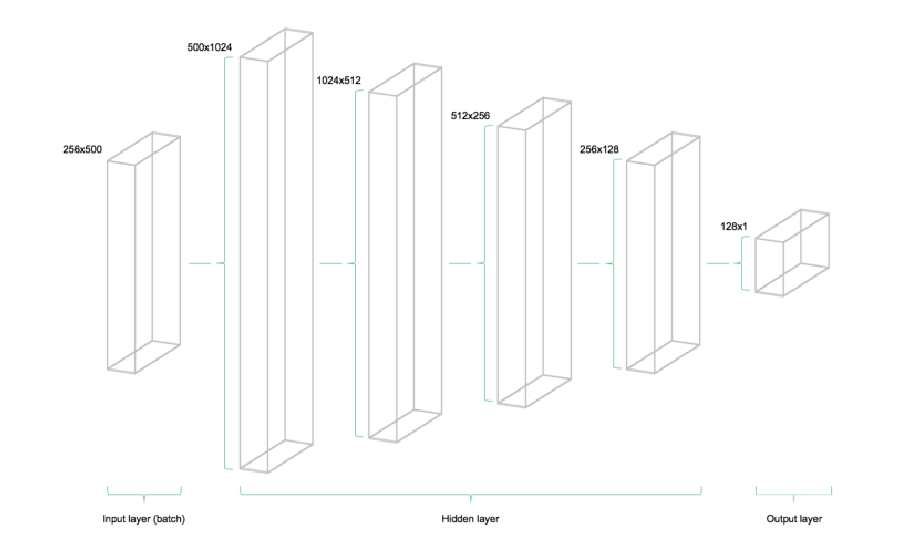
\includegraphics[scale=0.6]{/home/raghav/Desktop/stockprediction/02_code/NNf.eps}
\caption{Schematic of the Neural Network used}
\end{figure} 
Ultimately, the selection of architecture comes down to trial and error, and has no real rule of thumb, but the above choice of ours was the most straightforward logical trial.
\subsubsection{Choice of Gradient Descent}
There are various types of Gradient descent, ie: Batch Gradient Descent, Stochastic Gradient Descent, Mini Batch Gradient Descent etc.

The Stochastic Gradient Descent is a simple variant of classical gradient descent where the stochasticity comes from employing a random subset of the measurements (mini-batch) to compute the gradient at each descent. It also has implicit regularisation effects, making it suited for highly non-convex loss functions like in our case.

The Stochastic Gradient descent takes less computation time than it's other counterparts, and for this reason we choose it.

\section{Results}
We first plotted the S$\&$P 500 index over time as shown in Figure 4.
This is actually the lead of the S$\&$P 500 index, meaning, its value is shifted 1 minute into the future. This operation is necessary since we want to predict the next minute of the index and not the current minute. Each row in the dataset contains the price of the S$\&$P500 at t+1 and the constituent’s prices at T=t.
\begin{adjustbox}{center,caption={First 5 rows and 6 columns of the dataset},label={somelabel},nofloat=figure,vspace=\bigskipamount}
% maybe other stuff
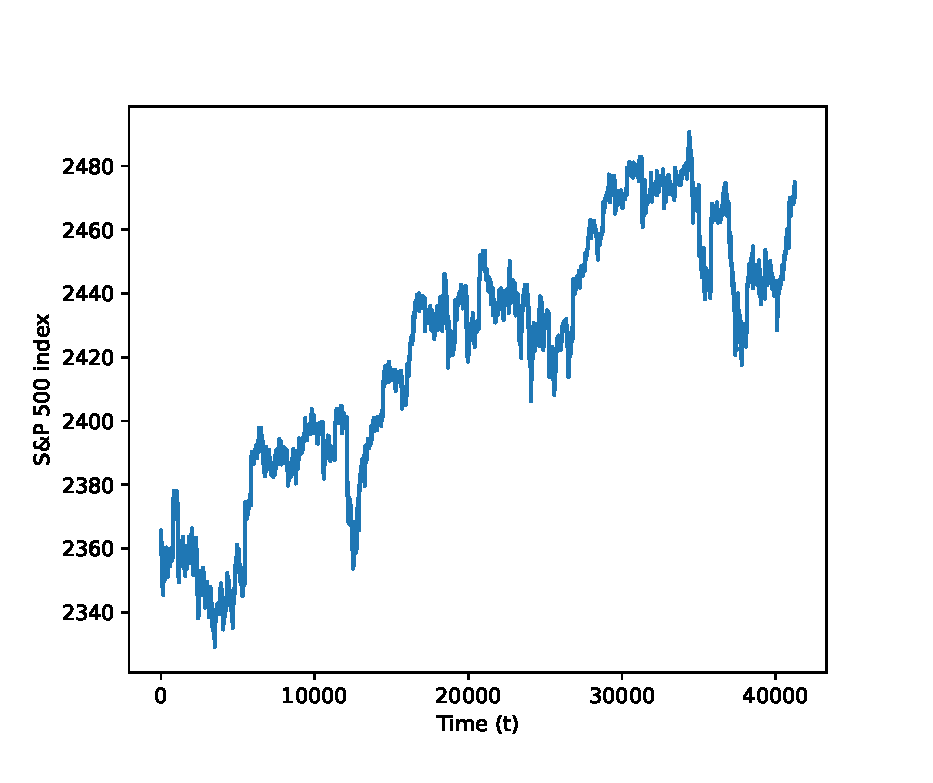
\includegraphics[scale = 0.6]{/home/raghav/Desktop/stockprediction/02_code/SP500.eps}% example only, could also be \adjustimage
% maybe other stuff
\end{adjustbox}
The data was then divided into batches and then passed on into the neural network where it \textit{learned} over the course of 10 \textbf{\textit{epochs}}. The following figures display the prediction of the neural network(in orange) plotted over the original plot of Figure 4.
\begin{figure}[!htb]
   \begin{minipage}{0.48\textwidth}
     \centering
     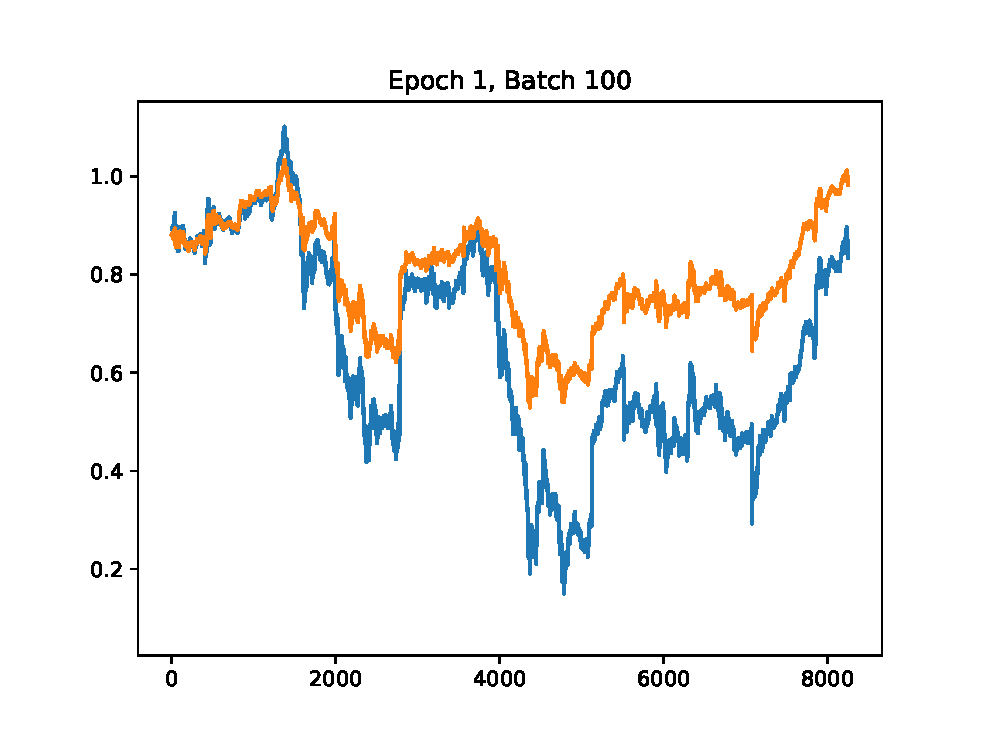
\includegraphics[scale = 0.4]{/home/raghav/Desktop/stockprediction/02_code/1.eps}
     \caption{Epoch 1 batch 100}\label{Fig:Data1}
   \end{minipage}\hfill
   \begin{minipage}{0.48\textwidth}
     \centering
     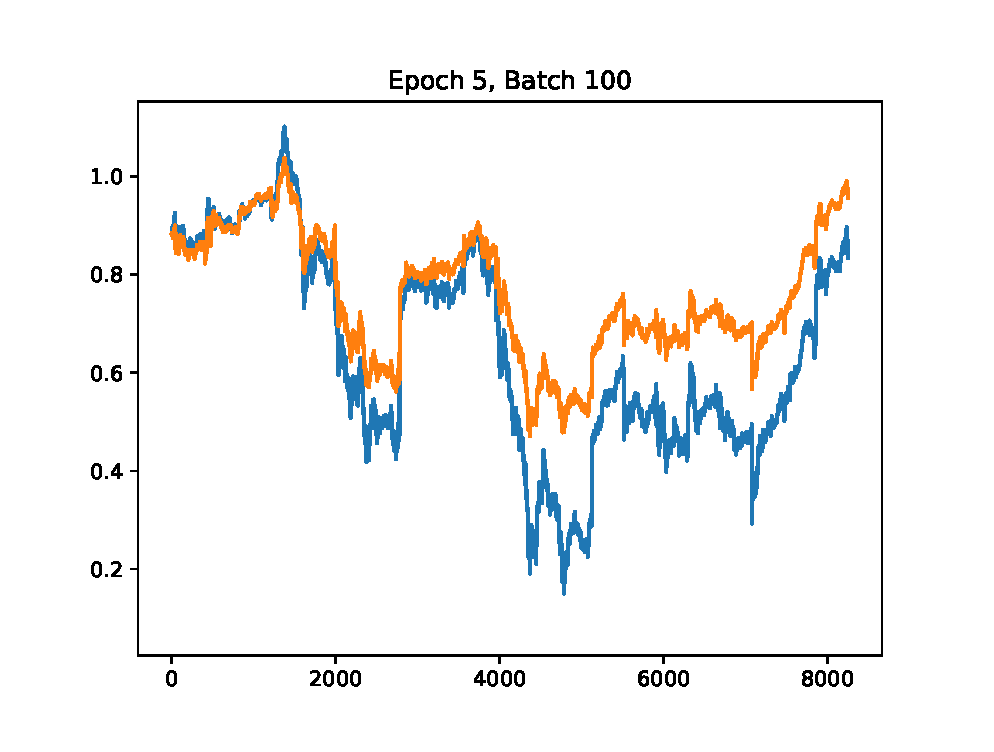
\includegraphics[scale = 0.4]{/home/raghav/Desktop/stockprediction/02_code/5.eps}
     \caption{Epoch 5 batch 100}\label{Fig:Data2}
   \end{minipage}
\end{figure}

\begin{figure}[!htb]
	\begin{minipage}{0.48\textwidth}
     \centering
     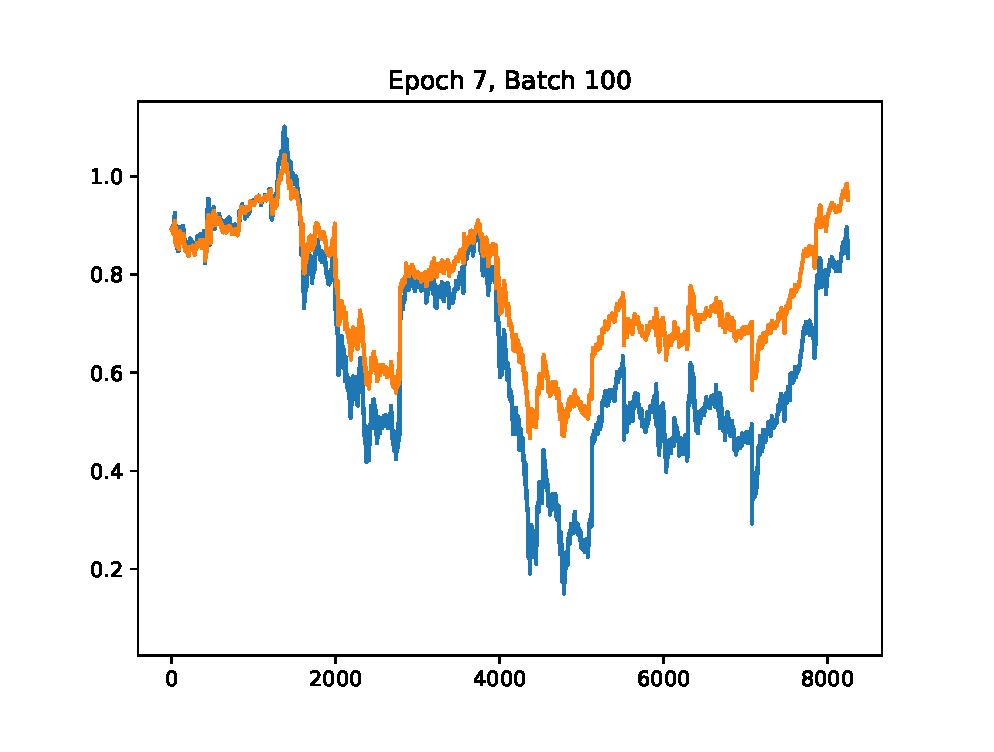
\includegraphics[scale = 0.4]{/home/raghav/Desktop/stockprediction/02_code/7.eps}
     \caption{Epoch 7 batch 100}\label{Fig:Data2}
   \end{minipage}
   \begin{minipage}{0.48\textwidth}
     \centering
     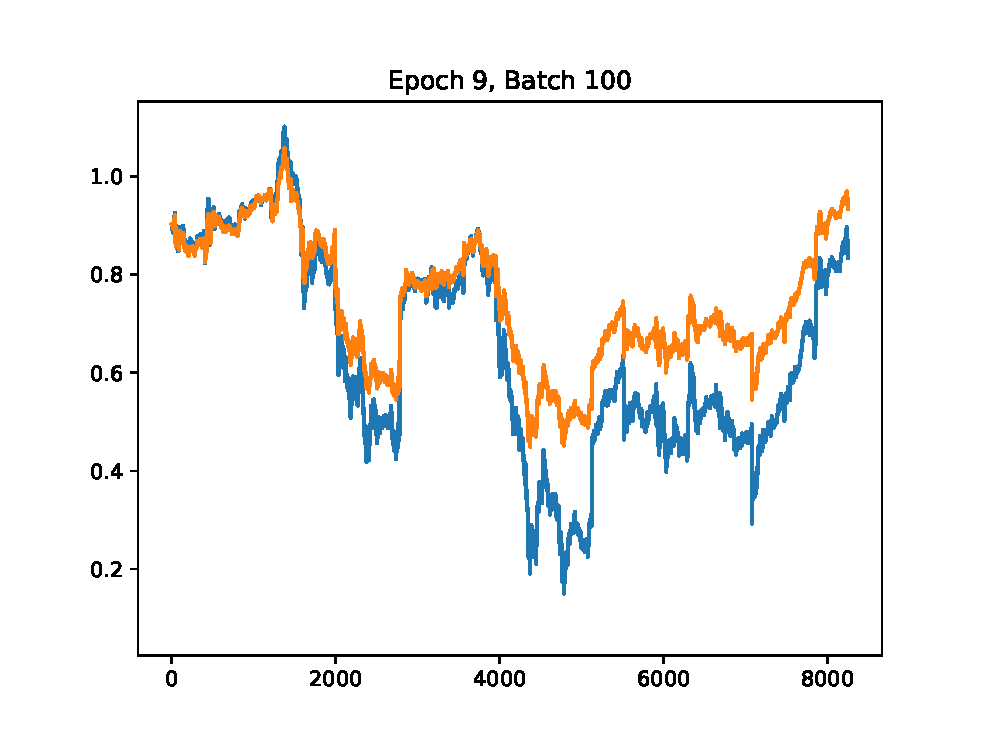
\includegraphics[scale = 0.4]{/home/raghav/Desktop/stockprediction/02_code/100.eps}
     \caption{Epoch 9 batch 100}\label{Fig:Data1}
   \end{minipage}\hfill
   
\end{figure}
As we see the prediction of the Neural Network (in orange) converges to the actual plot (in blue) near the end of the 10th epoch.
\newpage
\section{Conclusion}
The whole motivation behind this paper, was to use simple data manipulation tools and fairly simple data analysis theory to produce a strong real life application of the same.
Through the Predicted vs Actual figure shown above, we see that even though we are not exactly accurate, we have managed to make a decent guess with acceptable error margins.
\section{References}
\begin{itemize}
    \item https://www.heatonresearch.com/2017/06/01/hidden-layers.html
    \item https://arxiv.org/abs/1805.11317
    \item https://www.analyticsindiamag.com/how-stochastic-gradient-descent-is-solving-optimisation-problems-in-deep-learning/
    \item https://missinglink.ai/guides/neural-network-concepts/7-types-neural-network-activation-functions-right/
\end{itemize}
\footnote{All codes and figures can be found at https://github.com/ArcticSoup/Stock-Market-Analysis or https://github.com/Gautham-G/Market\_Analysis}
\end{document}